% ----------------------------------------------------------
% Introdução 
% Capítulo sem numeração, mas presente no Sumário
% ----------------------------------------------------------

\chapter*[Introdução]{Introdução}
\addcontentsline{toc}{chapter}{Introdução}

Este relatório descreve o método utilizado para o projeto de um sistema de rádio enlace ponto a ponto, com base nos dois pontos fornecidos.

Segundo TUDE, o enlace de rádio pode ser definido como : "
Uma aplicação da transmissão de informação por meio de ondas eletromagnéticas, se caracterizando como uma das aplicação que faz parte das Segundo Tude , “Um enlace rádio digital ponto a ponto é utilizado para o transporte de informação entre dois pontos fixos,tendo o espaço livre como meio de transmissão (wireless)”.[1]


\section*{Proposta}\label{sec:motivacao}

Projetar um sistema de rádio enlace ponto a ponto, entre os pontos mostrados nos mapas anexados.
\begin{figure}[!htb]
	\begin{minipage}{0.48\textwidth}
		\centering
		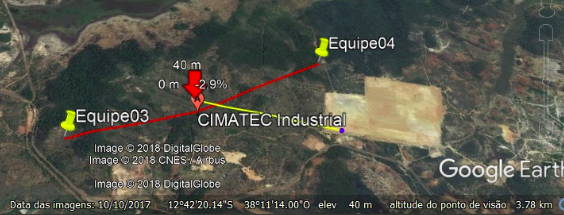
\includegraphics[width=1\linewidth]{ponto_a.png}
		\caption{Ponto A}\label{Fig:ponto_a_intro}
	\end{minipage}\hfill
	\begin{minipage}{0.48\textwidth}
		\centering
		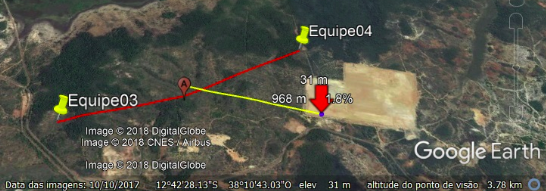
\includegraphics[width=1\linewidth]{ponto_b.png}
		\caption{Ponto B}\label{Fig:ponto_b_intro}
	\end{minipage}
\end{figure}

Foi solicitado que sejam tomadas as seguintes decisões:

\begin{itemize}
\item Definir a frequência de operação;
\item Calcular a Potência do Rádio Transmissor, Sensibilidade do Receptor e ganhos das Antenas, para o enlace fornecido;
\item Definir solução a ser adotada com base em fornecedores comerciais reais (Ex:
Intelbras, Ubiquiti, Tp Link, MikroTik, entre outros)
\end{itemize}

